\documentclass[12 pt]{article}
\usepackage[left=2.66cm,top=3cm,right=2.66cm,bottom=3cm,bindingoffset=0.5cm]{geometry}

\usepackage{graphicx}
\usepackage{setspace}
\usepackage{enumitem}
\onehalfspacing

\begin{document}
\begin{titlepage}
\begin{Huge}
\begin{center}
\textsc{ RSA Algorithm \linebreak
and \linebreak
Public Key Cryptosystems}
\end{center}
\end{Huge}
\begin{center}
\begin{large}
\textsl{ Rohan Datta, Divya Raj}
\end{large}
\end{center}

\bigskip 
\begin{center}
\textbf{Abstract}
\end{center}
This text discusses the concept behind public key cryptosystems, while focusing on a very popular encryption method. It interprets the algorithm into an accessible form. An array of real world implementations of the algorithm is also presented.\\[22 pt]
\noindent \textit{Key words and phrases:} cryptosystems, discrete mathematics, encryption, decryption, prime numbers, digital signatures, public key cryptosystems, authentication, cyber security.

\end{titlepage}
\pagebreak
\begin{LARGE}	
\begin{center}
\textbf{\textsc{Introduction to Public-Key Cryptography}}
\end{center}
\end{LARGE}

\noindent 
\\Public key cryptography, or asymmetrical cryptography, is any cryptographic system that uses pairs of keys: public keys which may be disseminated widely, and private keys which are known only to the owner. This accomplishes two functions: authentication, which is when the public key is used to verify that a holder of the paired private key sent the message, and encryption, whereby only the holder of the paired private key can decrypt the message encrypted with the public key.
\\\\The various methods that can and were used as alternatives to the public key systems are as follows:
\\\textbf{1. Symmetric}\\In a symmetric-key algorithm, both the sender and receiver share the key. The sender uses the key to hide the message. Then, the receiver will use the same key in the opposite way to reveal the message. For centuries, most cryptography has been symmetric. The problem with this system is that you have to make sure that the key is shared in a secure way, thus creating a chicken - egg dilemma.

\begin{figure}[h!]
  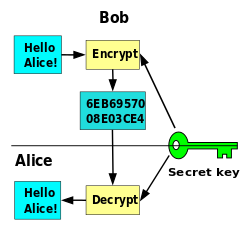
\includegraphics[width=60mm]{Symmetric_key_encryption.png}
  \centering
  \caption{Symmetric-key cryptography.}
  \label{fig:Symmetric-key cryptography}
\end{figure}
\noindent
\\\textbf{2. Decryption - Encryption in the middle}
\\In this system instead of having just two parties like above, one common third party(mostly a server) is added. So now, the sender and the server share a key(say K\textsubscript{a}), and the server and the receiver share a key(say K\textsubscript{b}). The sender's message is encrypted using K\textsubscript{a}, is decrypted at the server, then it is encrypted by K\textsubscript{b}, and sent to the receiver, where it finally gets decrypted and the message is delivered. The problem here is that the server becomes an obvious fail point, if its security is compromised, the whole system might fail.

\textbf{Hence the Public-Key system}, which is as follows:
\\
\noindent In a public key encryption system, any person can encrypt a message using the public key of the receiver, but such a message can be decrypted only with the receiver's private key. For this to work, it must be computationally easy for a user to generate a public and private key-pair to be used for encryption and decryption.

\begin{figure}[h!]
  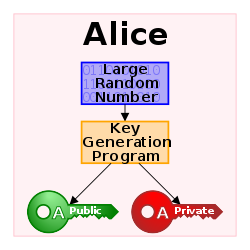
\includegraphics[width=50mm]{250px-Public-key-crypto-1.png}
  \centering
  \caption{A typically large and random number is used to begin generation of an acceptable pair of keys suitable for use by an asymmetric key algorithm.}
  \label{fig:PublicKey-NumGen}
\end{figure}

\noindent The strength of a public key cryptography system relies on the degree of difficulty (computational impracticality) for a properly generated private key to be determined from its corresponding public key. Security then depends only on keeping the private key private, and the public key may be published without compromising security.


\begin{figure}[h!]
  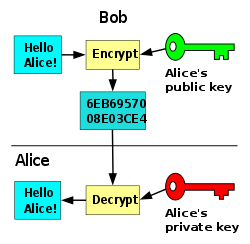
\includegraphics[width=50mm]{250px-Public_key_encryption.png}
  \centering
  \caption{The basic mechanism of a public key encryption system.}
  \label{fig:PublicKey-Basic}
\end{figure}

\noindent Public key cryptography systems often rely on cryptographic algorithms based on mathematical problems that currently admit no efficient solution — particularly those inherent in certain integer factorization, discrete logarithm, and elliptic curve relationships. Public key algorithms, unlike symmetric key algorithms, do not require a secure channel for the initial exchange of one (or more) secret keys between the parties.

\noindent Because of the computational complexity of asymmetric encryption, it is usually used only for small blocks of data, typically the transfer of a symmetric encryption key (e.g. a session key). This symmetric key is then used to encrypt the rest of the potentially long message sequence. The symmetric encryption/decryption is based on simpler algorithms and is much faster.

\noindent
Two of the best-known uses of public key cryptography are:

\begin{itemize}

\item \textbf{Public key encryption}, in which a message is encrypted with a recipient's public key. The message cannot be decrypted by anyone who does not possess the matching private key, who is thus presumed to be the owner of that key and the person associated with the public key. This is used in an attempt to ensure confidentiality.

An analogy to public key encryption is that of a locked mail box with a mail slot. The mail slot is exposed and accessible to the public – its location (the street address) is, in essence, the public key. Anyone knowing the street address can go to the door and drop a written message through the slot. However, only the person who possesses the key can open the mailbox and read the message.
\\
\item \textbf{Digital signatures}, in which a message is signed with the sender's private key and can be verified by anyone who has access to the sender's public key. This verification proves that the sender had access to the private key, and therefore is likely to be the person associated with the public key. This also ensures that the message has not been tampered with, as a signature is mathematically bound to the message it originally was made with, and verification will fail for practically any other message, no matter how similar to the original message.


An analogy for digital signatures is the sealing of an envelope with a personal wax seal. The message can be opened by anyone, but the presence of the unique seal authenticates the sender.
\end{itemize}

\pagebreak

\begin{Large}
\noindent \textbf{{Uses of Public-key Cryptography}}
\end{Large}\\[12pt]

\noindent Public key cryptography is often used to secure electronic communication over an open networked environment such as the Internet, without relying on a hidden or covert channel, even for key exchange. Open networked environments are susceptible to a variety of communication security problems, such as man-in-the-middle attacks and spoofs. \\[6pt]
Communication security typically includes requirements that the communication must not be readable during transit (preserving confidentiality), the communication must not be modified during transit (preserving the integrity of the communication), the communication must originate from an identified party (sender authenticity), and the recipient must not be able to repudiate or deny receiving the communication. Combining public key cryptography with an Enveloped Public Key Encryption (EPKE) method, allows for the secure sending of a communication over an open networked environment. In other words, even if an adversary listens to an entire conversation including the key exchange, the adversary would not be able to interpret the conversation.

\emph{\\\\There are various algorithms which are employed to generate and implement the public and private key, one of them the RSA algorithm, which will be elucidated upon in the next section.}

\pagebreak
\begin{LARGE}	
\begin{center}
\textbf{\textsc{RSA Algorithm}}
\end{center}
\end{LARGE}

\noindent RSA algorithm is an asymmetric cryptographic algorithm that is used extensively by computers nowadays. It was proposed by Ron Rivest, Adi Shamir and Leonard Adleman in their 1978 paper \textsuperscript{[1]}, and hence, bears their name. It is one of the most popular implementations of public key cryptosystems.\bigskip

\noindent It is built on the fact that finding the prime factors of a number is one of the most complex mathematical problems \textsuperscript{[2]}. Initially, the user creates and publishes the product of two large prime numbers, along with an auxiliary value. The auxiliary value takes up the role of the ``public key'' which is known to all. \emph{But, the prime factors must be kept secret.}\bigskip

1. Choose\ two\ different,\ large,\ random\  prime\  numbers\ \textbf{p} and \textbf{q}

2. Calculate \textbf{n} = \textbf{p}*\textbf{q}

3. \textbf{\boldmath $\phi(n)$ = (p - 1)*(q - 1)}

4. Choose an integer \textbf{e} such that:\\[3 pt]

\hspace{16.18 pt} $\bullet$ \textbf{1} \textless \textbf{e} \textless \boldmath $\phi(n)$, and

\hspace{16.18 pt} {$\bullet$ \textbf{e} is co-prime to \boldmath $\phi(n)$\\[3 pt]

5. Compute \textbf{d} such that \boldmath \textbf{d}*\textbf{e} = 1+\textbf{k}*\boldmath $\phi(n)$
\bigskip
\\
A popular choice for public exponents is \textbf{e} = $2$ \textsuperscript{$16$}+$1 = 65537$\bigskip

\noindent The public key is made of the modulus \textbf{n} and the public (or encryption) exponent \textbf{e}.

\noindent The private key is made of the modulus \textbf{n} and the private (or decryption) exponent \textbf{d} which must be kept secret.

\pagebreak

\begin{LARGE}
\noindent \textbf{How encryption is done}
\end{LARGE}\\[12 pt]

\noindent Person A, say, Alice gives her public key ($n,e$) to Person B, say, Bob and keeps her private key secret. Bob wants to send a message \textbf{M} to Alice.

\noindent So, first, he turns \textbf{M} into a number \textbf{m} smaller than \textbf{n}, by using an agreed-upon reversible protocol known as ``padding scheme"(\emph{see below}). He then computes the ciphertext \textbf{c} corresponding to:

$c = m$\textsuperscript{$e$} $mod$ $n$
\bigskip

\noindent This ciphertext is then sent to Alice.
\\[22 pt]

\begin{LARGE}
\noindent \textbf{How decryption is done}
\end{LARGE}\\[12 pt]

\noindent Alice can recover \textbf{m} from c by using her private key, \textbf{d} in the following way: \bigskip

$m = c$\textsuperscript{$d$} $mod$ $n$
\bigskip

\noindent Given m, she can recover the original, distinct, prime numbers, in the following way: \bigskip

$m$\textsuperscript{$ed$} $\equiv$ $m$ \hspace{66 pt} ($mod$ $pq$)\bigskip

Thus, \bigskip

$c$\textsuperscript{$d$} $\equiv$ $m$ \hspace{66 pt} ($mod$ $n$)
\\[10 pt]

\noindent Using this, $m$ is calculated. Then, using the padding scheme, $m$ is converted back to $M$, which was the original message.
\pagebreak

\begin{LARGE}
\noindent \textbf{Padding Scheme}
\end{LARGE}\\[12 pt]

\noindent Very often, messages start or end in a well-known way (Dear Bob, ..., Yours, Alice ). This is a problem, because that knowledge could be used to break (or start to break) encryption. To prevent this, a number of random characters are added at the beginning or the end of the message. This procedure is called ``padding".
\\

\noindent When used in practice, RSA must be combined with some form of padding scheme, so that no values of M result in insecure ciphertexts. Most practical RSA implementations typically embed some form of structured, randomized padding into the value $m$ before encrypting it. This padding ensures that $m$ does not fall into the range of insecure plaintexts, and that a given message, once padded, will encrypt to one of a large number of different possible ciphertexts. The latter property can increase the cost of a dictionary attack beyond the capabilities of a reasonable attacker. Modern contructions use secure techniques such as Optimal Asymmetric Encryption Padding (OAEP) to protect messages while preventing these attacks. \\[16.18pt]

\begin{LARGE}
\noindent \textbf{Digital Signature}
\end{LARGE}\\[12 pt]

\noindent Suppose Alice uses Bob's public key to send him an encrypted message. In the message, she can claim to be Alice but Bob has no way of verifying that the message was actually from Alice since anyone can use Bob's public key to send him encrypted messages. So, in order to verify the origin of a message, RSA can also be used to authenticate a message.\\

\noindent So, Alice produces a hash value of the message, raises it to the power of d mod n, and attaches it as a ``signature" to the message. When Bob receives the signed message, he raises the signature to the power of e mod n, and compares the resulting hash value with the message's actual hash value. If the two match, he knows that the author of the message was in possession of Alice's secret key, and that the message has not been tampered with since. So, the author must be Alice.

\pagebreak

\begin{LARGE}
\noindent \textbf{Real World Applications of RSA Algorithm}
\end{LARGE}\\[12 pt]
The RSA Algorithm is utilized extensively for many practical applications. Typically, these applications can be categorized as "key exchange" and/or "digital signature".
\\\\\textbf{HTTPS is implimented usng RSA.}
\\For example, when we visit a website beginning with "https://", it is highly likely that the web browser is using RSA to validate the certificate for the remote server to which we have connected. Once the browser validates the certificate chain (using RSA signature functionality), it will probably use RSA to perform a secure key exchange with the server. The end result: the browser can communicate securely with a remote server and provide us with confidence that the remote server in question is indeed the server you intended to contact -- and not an intruder executing a man-in-the-middle attack to steal private information.
\\\\HTTPS is used with countless websites where the exchange of personal or private information takes place (passwords, eCommerce, etc.)
\\\\Computer applications are often digitally signed so that the consumer can verify that the software has not been modified since the publisher released it. If the software is modified after signing (even by one bit) the digital signature will fail. This provides a way to prevent non-trusted code from executing.
\\\\Then there are other technologies like commercial satellite radio, satellite TV, etc. If the content publisher simply broadcast the media in the clear, they would have a difficult time convincing people to pay their monthly bill. Instead they need a means to distribute the decryption keys to their paid subscribers, while keeping the general public out -- RSA is a candidate for that too.
\\\\RSA is used for many other \textbf{Digital Rights Management} (DRM) applications. DRM is a set of access control technologies for restricting the use of proprietary hardware and copyrighted works. DRM technologies try to control the use, modification, and distribution of copyrighted works (such as software and multimedia content), as well as systems within devices that enforce these policies.
\\\\The security of the RSA Algorithm is based on the belief that factoring large integers is and will continue to be computationally expensive. RSA has been in use for more than 30 years and to this day is still considered secure, provided keys of sufficient length are used. Keys created today are typically at least 2048 bits.
\\\\\textbf{Why is RSA so popular?}
\begin{itemize}
  \item It's not governed by any active patents.
  \item Anyone can use it, royalty free in any private or commercial
 product.
 \item RSA can do encryption, decryption, signature and signature verification -- all with the same two functions.
 \item It has been around for more than 30 years and has not been compromised.
\end{itemize} 


\pagebreak

\begin{large}
\begin{center}
\textbf{References and Citations}\\[16pt]
\end{center}
\end{large}

\begin{enumerate}
\item Rivest, Shamir, Adleman. A Method for Obtaining Digital Signatures and Public-Key Cryptosystems (1978)
\item Crow. Prime Numbers in Public Key Cryptography - An Introduction 
\item Levine, J., and Brawley, J.V. Some cryptographic applications of permutation polynomials (1977)
\item Rivest, et al. United States Patent: 4405829
\item National Archives And Records Administration. Federal Register: 40 Fed. Reg. 12067 Mar. 17, 1975
\end{enumerate}

\end{document}